\hypertarget{explorer_8cpp}{}\section{/home/srinidhi/catkin\+\_\+ws/src/et\+\_\+exploration\+\_\+robot/src/explorer.cpp File Reference}
\label{explorer_8cpp}\index{/home/srinidhi/catkin\+\_\+ws/src/et\+\_\+exploration\+\_\+robot/src/explorer.\+cpp@{/home/srinidhi/catkin\+\_\+ws/src/et\+\_\+exploration\+\_\+robot/src/explorer.\+cpp}}


\hyperlink{classExplorer}{Explorer} class method definitions.  


{\ttfamily \#include $<$actionlib/client/simple\+\_\+action\+\_\+client.\+h$>$}\\*
{\ttfamily \#include $<$geometry\+\_\+msgs/\+Pose.\+h$>$}\\*
{\ttfamily \#include $<$move\+\_\+base\+\_\+msgs/\+Move\+Base\+Action.\+h$>$}\\*
{\ttfamily \#include $<$nav\+\_\+msgs/\+Occupancy\+Grid.\+h$>$}\\*
{\ttfamily \#include $<$ros/ros.\+h$>$}\\*
{\ttfamily \#include $<$cmath$>$}\\*
{\ttfamily \#include $<$cstdint$>$}\\*
{\ttfamily \#include $<$limits$>$}\\*
{\ttfamily \#include $<$utility$>$}\\*
{\ttfamily \#include $<$vector$>$}\\*
{\ttfamily \#include \char`\"{}et\+\_\+exploration\+\_\+robot/explorer.\+hpp\char`\"{}}\\*
{\ttfamily \#include \char`\"{}et\+\_\+exploration\+\_\+robot/grid.\+hpp\char`\"{}}\\*
{\ttfamily \#include \char`\"{}et\+\_\+exploration\+\_\+robot/map.\+hpp\char`\"{}}\\*
Include dependency graph for explorer.\+cpp\+:
\nopagebreak
\begin{figure}[H]
\begin{center}
\leavevmode
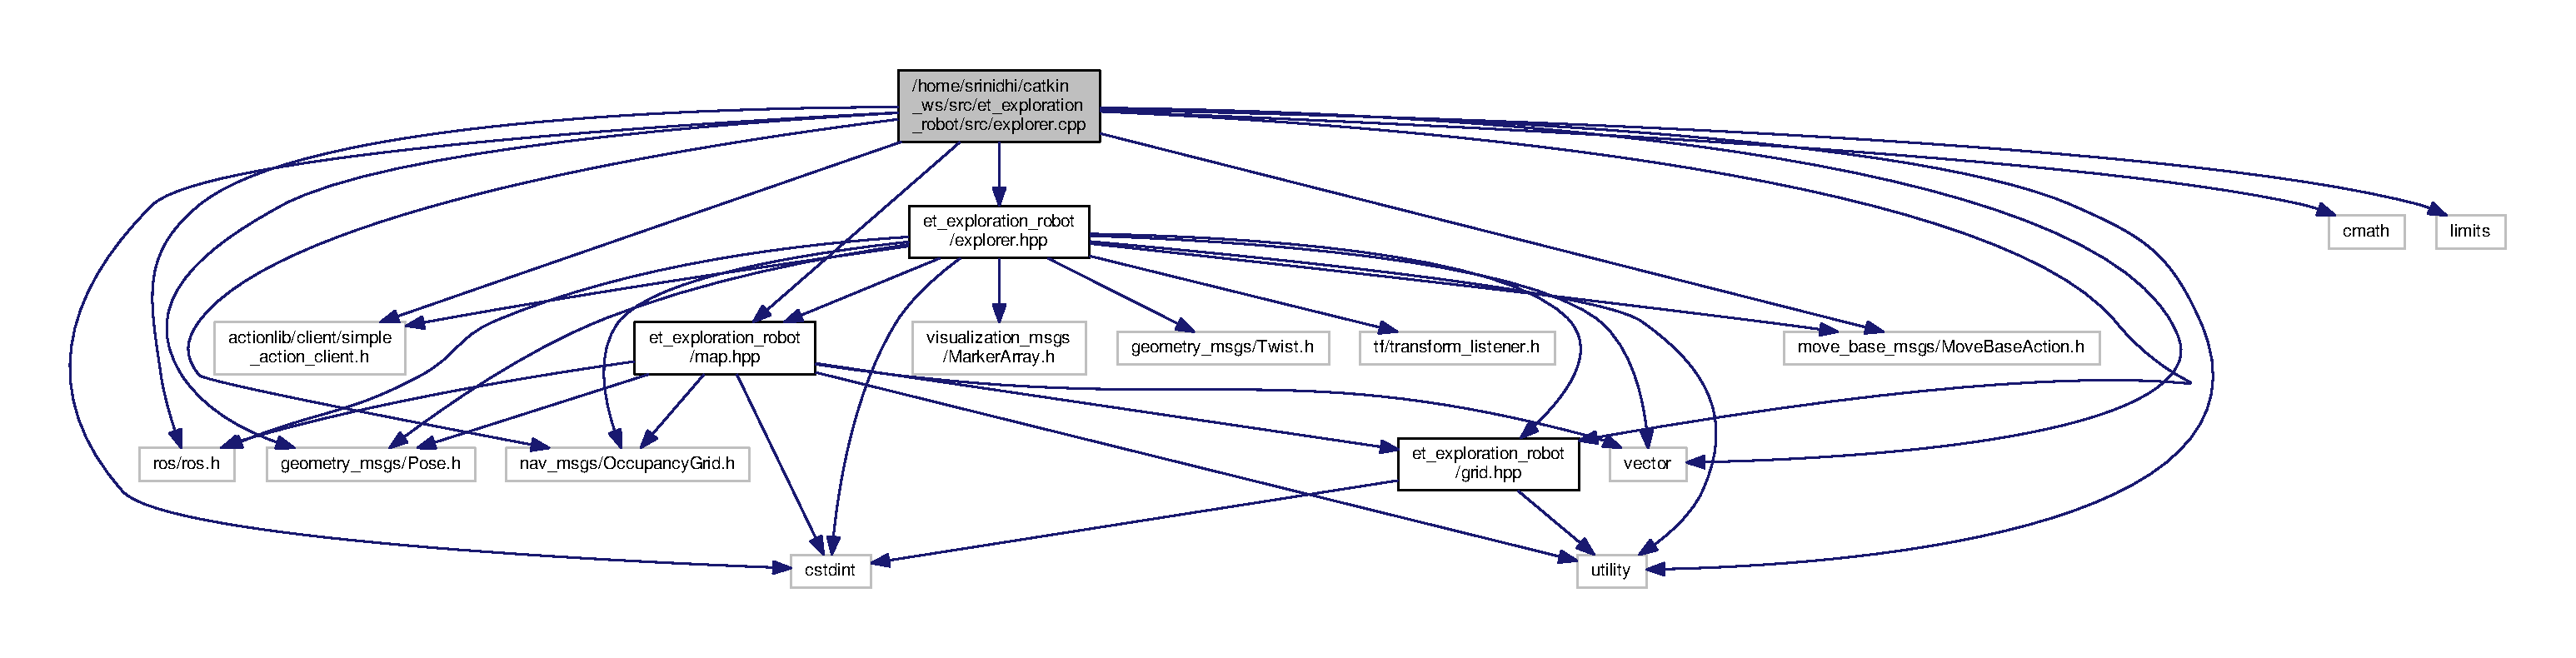
\includegraphics[width=350pt]{explorer_8cpp__incl}
\end{center}
\end{figure}


\subsection{Detailed Description}
\hyperlink{classExplorer}{Explorer} class method definitions. 

\begin{DoxyAuthor}{Author}
Srinidhi Sreenath (Srinidhi\+Sreenath) 
\end{DoxyAuthor}
\begin{DoxyDate}{Date}
12/15/2018 
\end{DoxyDate}
\begin{DoxyVersion}{Version}
1.\+0
\end{DoxyVersion}
\hypertarget{mapTest_8cpp_DESCRIPTION}{}\subsection{D\+E\+S\+C\+R\+I\+P\+T\+I\+ON}\label{mapTest_8cpp_DESCRIPTION}
Source file for class \hyperlink{classExplorer}{Explorer} which implements the exploration behavior for a turtlebot in an unknown environment. The turtlebot intially rotates in the environment and determines the frontiers i.\+e regions between explored and unexplored regions. It then navigates to closest reachable frontier and then restarts the rotation behavior to determine new frontiers. The behavior continues until the exploration is complete. 